De acordo com a Lei Universal da Gravita��o, proposta por Isaac Newton, a intensidade da for�a gravitacional F que a Terra exerce sobre um sat�lite em �rbita circular � proporcional � massa $m$ do sat�lite e inversamente proporcional ao quadrado do raio $r$ da �rbita, ou seja
\begin{equation*}
F=\frac{K.m}{r^2}
\end{equation*}
No Plano cartesiano, tr�s sat�lites A, B e C, est�o representados, cada um, por um ponto (m; r) cujas coordenadas s�o, respectivamente, a massa do sat�lite e o raio da sua �rbita em torno da Terra
\begin{figure}[h]
\caption{Exemplo}
\centering
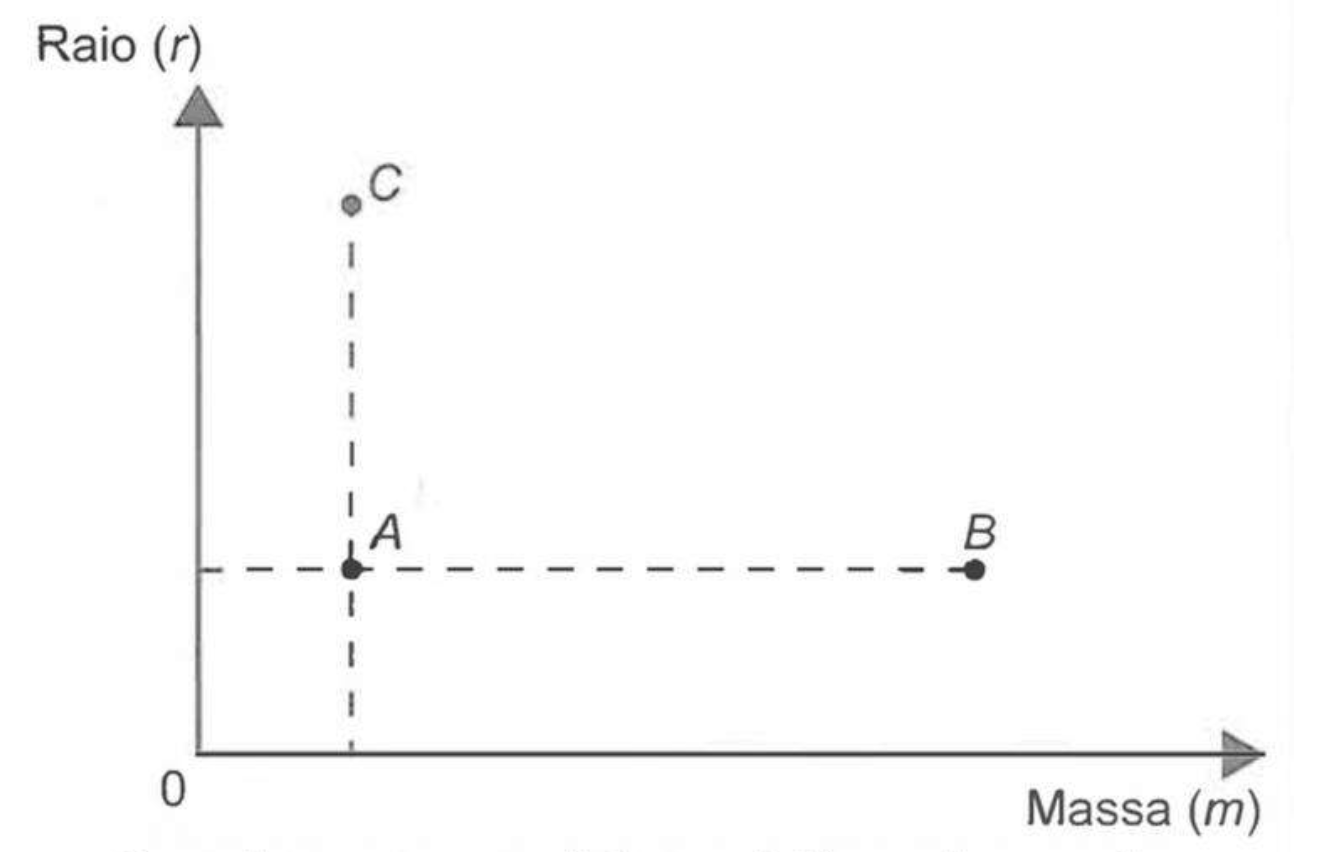
\includegraphics[width=8cm]{../figuras/q136-2018.png}
\label{Figura:1}
\end{figure}
Com base nas posi��es relativas dos pontos no gr�fico, deseja-se comparar as intensidades $F_A$, $F_B$, e $F_C$ expressas no gr�fico satisfazem a rela��o
\begin{enumerate}
\item[a)] $F_C=F_A < F_B$
\item[b)]$F_A=F_B < F_C$
\item[c)]$F_A<F_B < F_C$
\item[d)]$F_A<F_C < F_B$
\item[e)]$F_C<F_A < F_B$
\end{enumerate}